\documentclass[12pt]{article}
\usepackage{geometry}
\usepackage{titlesec}
\usepackage{enumitem}
\usepackage{tabularx}
\usepackage{color, hyperref, xcolor}
\usepackage[document]{ragged2e}
\usepackage{xtab}
\usepackage{graphicx}
\usepackage{multirow}
\geometry{paperheight=11in, paperwidth=8.5in, margin=1cm}
\thispagestyle{empty}

\newcommand{\resumename}[1]{\LARGE\textbf{#1} \hfill \small}

\titleformat{\section}
  {\normalfont\fontsize{12pt}{14pt}\bfseries}{\thesection}{1em}{}[{\titlerule[0.8pt]}]

\titlespacing*{\section}{0em}{0.5em}{0.5em}
\titleformat{\subsection}[runin]{\bfseries}{}{}{}[]
\titlespacing*{\subsection}{0em}{0.5em}{0em}

\begin{document}
\noindent
\resumename{Akanksha Bhadauria}

\begin{table}[h]
    \hspace*{-10pt}
    \begin{tabular}{llrp{0cm}}
        \multirow{1}{*}{\textbf{LinkedIn}} & \multirow{1}{*}{\href{https://www.linkedin.com/in/bhadauriakanksha2403/}{linkedin.com/in/bhadauriakanksha2403/}} &
        \multirow{1}{*}{\hspace*{1.5cm} Email: \href{mailto:bhadauriakanksha2403@gmail.com}{bhadauriakanksha2403@gmail.com}} & \multirow{4}{*}{
            % 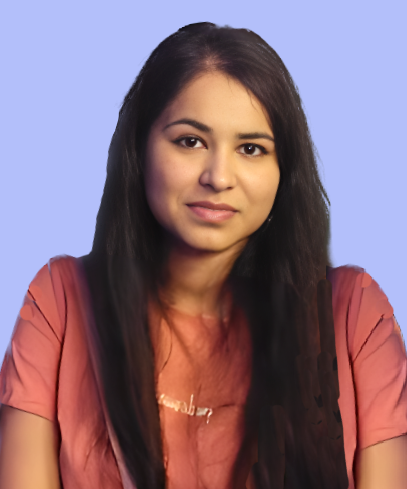
\includegraphics[width=2.0cm]{akanksha_photo.png}
        } \\
        \multirow{1}{*}{\textbf{GitHub}}   & \multirow{1}{*}{\href{https://github.com/akanksha2403}{github.com/akanksha2403}}                                 & \multirow{1}{*}{Mobile: \href{tel:+918433434933}{+91-8433434933}} \\
        \textbf{Codechef}                  & \href{https://www.codechef.com/users/tanishka125}{codechef.com/users/tanishka125}                                &                                                                   \\
        \textbf{Codeforces}                & \href{https://codeforces.com/profile/tanu24}{codeforces.com/profile/tanu24}                                      &                                                                   \\
    \end{tabular}
\end{table}

\vspace{-\topsep}
\section*{EDUCATION}
\subsection*{Indian Institute of Information Technology, Lucknow} \hfill \textbf{Lucknow, Uttar Pradesh, India} \\
Bachelor of Technology - Information Technology (CGPA: 7.72/10) \hfill \textit{December 2020 - Present (May 2024)} \\
\subsection*{John Milton Public School} \hfill \textbf{Agra, Uttar Pradesh, India} \\
CBSE Class 10\textsuperscript{th} \& 12\textsuperscript{th} (10\textsuperscript{th} Percentage: 94\%, 12\textsuperscript{th} Percentage: 95.6\%) \hfill \textit{December 2016 - June 2020}

\section*{PROJECTS}
\subsection*{\href{https://github.com/Akanksha2403/no_issues}{No Issues}}~ Django $\vert$ Data Structures $\vert$ CSS $\vert$ JavaScript $\vert$ Bootstrap $\vert$ Perspective API\\
\begin{itemize}[leftmargin=20px, topsep=1pt, itemsep=1.5pt, partopsep=1pt, parsep=1pt]
  \item Developed a web-based Complaint Management System which have automatic complaint escalation to higher authorities based on response deadlines, enhancing workflow efficiency and ensuring timely resolution.
  \item Designed a database schema with a tree structure, utilizing self-referential foreign keys for efficient designation hierarchy management.
  \item Implemented user authentication to ensure secure access to the system.
  \item Incorporated offensive content detection mechanisms in complaint forms to prevent inappropriate submissions.
\end{itemize}

\subsection*{\href{https://akanksha2403.pythonanywhere.com/}{ShopApp}}~ Django $\vert$ HTML $\vert$ CSS $\vert$ JavaScript $\vert$ Bootstrap \\
\begin{itemize}[leftmargin=20px, topsep=0.5pt, itemsep=1.5pt, partopsep=0.5pt, parsep=0.5pt]
  \item Developed a dummy shop app that allows users to browse and purchase items online, similar to Amazon.
  \item Users can add items to cart, order, or track orders on the website.
  \item Created schema in database for storing information about products, orders, and users as well as for tracking order.
\end{itemize}
\subsection*{Machine Learning Datasets}~ Python $\vert$ Pandas $\vert$ Scikit-Learn $\vert$ Matplotlib $\vert$ Seaborn \\
\begin{itemize}[leftmargin=20px, topsep=0.5pt, itemsep=1.5pt, partopsep=0.5pt, parsep=0.5pt]
    \item Conducted a variety of hands-on machine learning projects by working on different datasets.
    \item Cleaned raw data using NumPy and Pandas and created visualizations using Matplotlib and Seaborn and used Scikit-Learn to train ML models respectively.
\end{itemize}


\section*{ACHIEVEMENTS}
\begin{itemize}[leftmargin=15px, topsep=1pt, itemsep=1pt, partopsep=2pt, parsep=2pt]
    \item Rated \textbf{4 stars} on \textbf{CodeChef} (Max rating: \textbf{1987}).
    \item Rated \textbf{Specialist} on \textbf{Codeforces} (Max rating: \textbf{1520}).
    \item Selected for \textbf{Amazon ML Summer School 2023}.
    \item Reached for finals in HackOFiesta v2.0 Equinox 2021 conducted by IIIT Lucknow.
    \item Global rank \textbf{32} in \href{https://www.codechef.com/rankings/START64B?search=tanishka125}{\textbf{CodeChef Starters 64 (Div. 2)}}.
    \item Global rank \textbf{78} in \href{https://www.codechef.com/rankings/START19C?search=tanishka125}{\textbf{CodeChef Starters 19 (Div. 3)}}.
    \item Global rank \textbf{207} in \href{https://www.codechef.com/rankings/START62B?search=tanishka125}{\textbf{CodeChef Starters 62 (Div. 2)}}.
    \item Global rank \textbf{386} in \href{https://codeforces.com/contest/1833/standings/participant/155663820#p155663820}{\textbf{Codeforces Round 874 (Div. 3)}}.
    \item Global rank \textbf{772} in \href{https://codeforces.com/contest/1816/standings/participant/153504271#p153504271}{\textbf{Codeforces Round 865 (Div. 2)}}.
    \item Global rank \textbf{928} in \href{https://codeforces.com/contest/1798/standings/participant/152498821#p152498821}{\textbf{Codeforces Round 860 (Div. 2)}}.
    \item Global rank \textbf{2467} in \href{https://codingcompetitions.withgoogle.com/kickstart/submissions/00000000008cb409/0000000000648019}{\textbf{Google Kickstart 2022 Round F}}.

\end{itemize}

\section*{TECHNICAL SKILLS}
\vspace{-2pt}
\begin{tabularx}{\textwidth}{@{}ll}
    \textbf{Languages}               & C/C++, Python                                                       \\
    \textbf{Frameworks \& Libraries} & Django, NumPy, Pandas, Scikit-learn, Bootstrap, Matplotlib, Seaborn \\
    \textbf{Dev Tools}               & Git/GitHub, VS Code, Jupyter Notebook                               \\
    \textbf{Academic Coursework}     & DSA, Operating System, OOPS, DBMS, Computer Networks                \\
\end{tabularx}

\end{document}
